%%%%%%%%%%%%%%%%%%%%%%%%%%%%%%%%%%%%%%%%%%%%%%%%%%%%%%%%%%%%%%%%%
% MUW Presentation
% LaTeX Template
% Version 1.0 (27/12/2016)
%
% License:
% CC BY-NC-SA 4.0 (http://creativecommons.org/licenses/by-nc-sa/3.0/)
%
% Created by:
% Nicolas Ballarini, CeMSIIS, Medical University of Vienna
% nicoballarini@gmail.com
% http://statistics.msi.meduniwien.ac.at/
%
% Customized for UAH by:
% David F. Barrero, Departamento de Automática, UAH
%%%%%%%%%%%%%%%%%%%%%%%%%%%%%%%%%%%%%%%%%%%%%%%%%%%%%%%%%%%%%%%%%

\documentclass[10pt,compress]{beamer} % Change 10pt to make fonts of a different size
\mode<presentation>

\usepackage[spanish]{babel}
\usepackage{fontspec}
\usepackage{tikz}
\usepackage{etoolbox}
\usepackage{xcolor}
\usepackage{xstring}
\usepackage{listings}

\usetheme{UAH}
\usecolortheme{UAH}
\setbeamertemplate{navigation symbols}{}
\setbeamertemplate{caption}[numbered]

%%%%%%%%%%%%%%%%%%%%%%%%%%%%%%%%%%%%%%%%%%%%%%%%%%%%%%%%%%%%%%%%%
%% Presentation Info
\title[Git]{Short Introduction to SCM and Git}
\author{D. Rodríguez, D. F. Barrero}
\institute{University of Alcalá}
\date{}
%%%%%%%%%%%%%%%%%%%%%%%%%%%%%%%%%%%%%%%%%%%%%%%%%%%%%%%%%%%%%%%%%


%%%%%%%%%%%%%%%%%%%%%%%%%%%%%%%%%%%%%%%%%%%%%%%%%%%%%%%%%%%%%%%%%
%% Descomentar para habilitar barra de navegación superior
\ponerNavegacion
%%%%%%%%%%%%%%%%%%%%%%%%%%%%%%%%%%%%%%%%%%%%%%%%%%%%%%%%%%%%%%%%%

%%%%%%%%%%%%%%%%%%%%%%%%%%%%%%%%%%%%%%%%%%%%%%%%%%%%%%%%%%%%%%%%%
%% Configuración de logotipos en portada
%% Opacidad de los logotipos
\newcommand{\opacidad}{1}
%% Descomentar para habilitar logotipo en pié de página de portada
\renewcommand{\logoUno}{Images/isg.png}
%% Descomentar para habilitar logotipo en pié de página de portada
%\renewcommand{\logoDos}{Images/CCLogo.png}
%% Descomentar para habilitar logotipo en pié de página de portada
%\renewcommand{\logoTres}{Images/ALogo.png}
%% Descomentar para habilitar logotipo en pié de página de portada
%\renewcommand{\logoCuatro}{Images/ELogo.png}
%%%%%%%%%%%%%%%%%%%%%%%%%%%%%%%%%%%%%%%%%%%%%%%%%%%%%%%%%%%%%%%%%

%%%%%%%%%%%%%%%%%%%%%%%%%%%%%%%%%%%%%%%%%%%%%%%%%%%%%%%%%%%%%%%%%
%% FOOTLINE
%% Comment/Uncomment the following blocks to modify the footline
%% content in the body slides.


%% Option A: Title and institute
\footlineA
%% Option B: Author and institute
%\footlineB
%% Option C: Title, Author and institute
%\footlineC
%%%%%%%%%%%%%%%%%%%%%%%%%%%%%%%%%%%%%%%%%%%%%%%%%%%%%%%%%%%%%%%%%

\begin{document}

%%%%%%%%%%%%%%%%%%%%%%%%%%%%%%%%%%%%%%%%%%%%%%%%%%%%%%%%%%%%%%%%%
% Use this block for a blue title slide with modified footline
{\titlepageBlue
    \setbeamertemplate{headline}{}
	\setbeamercolor{frametitle}{bg=black}
	\setbeamercolor{normal text}{bg=black}
    \begin{frame}
        \titlepage
    \end{frame}
}

\begin{frame}[plain]{}
   \begin{block}{Objectives}
      \begin{enumerate}
         \item Understand the need of SCM
         \item Implement software development workflows with Git and Github
      \end{enumerate}
   \end{block}

   %\begin{block}{Bibliography}
   %   \begin{enumerate}
   %       \item The Java\textsuperscript{TM} Tutorials. Oracle. \href{https://docs.oracle.com/javase/tutorial/}{(Link)}
   %   \end{enumerate}
   %\end{block}


\end{frame}

{
\eliminarNavegacion
\begin{frame}[shrink]{Table of Contents}
 \frametitle{Table of Contents}
 \tableofcontents
  % You might wish to add the option [pausesections]
\end{frame}
}

\section{Software Configuration Management (SCM)}

%%%%%%%%%%%%%%%%%%%%%%%%%%%%%%%%%%%%%%%%%%%%%%%%%%%%%%%%%%%%%%%%%%%%%%

\subsection{Version Control}


%%%%%%%%%%%%%%%%%%%%%%%%%%%%%%%%%%%%%%%%%%%%%%%%%%%%%%%%%%%%%%%%%%%%%%

\begin{frame}{Software Configuration Management (SCM)}{Version Control}

Version control systems (VCS) keep track of changes to source code.
Allows multiple people to edit a project in a predictable manner.

\end{frame}


%%%%%%%%%%%%%%%%%%%%%%%%%%%%%%%%%%%%%%%%%%%%%%%%%%%%%%%%%%%%%%%%%%%%%%

\subsection{Source Configuration Management}

%%%%%%%%%%%%%%%%%%%%%%%%%%%%%%%%%%%%%%%%%%%%%%%%%%%%%%%%%%%%%%%%%%%%%%

\begin{frame}[plain]{Software configuration Management (SCM)}{Source Configuration Management}


Software configuration management is the task of tracking and controlling changes in the software, part of the larger cross-disciplinary field of configuration management.\\
(\begin{scriptsize}\texttt{https://en.wikipedia.org/wiki/Software\_configuration\_management}                                                                                         \end{scriptsize})

Main open source software configuration management systems
\begin{itemize}
 \item 1982 RCS
 \item 1990 CVS
 \item 2000 Subversion
 \item 2005 Git/Mercurial
\end{itemize}

There are many proprietary ones but \texttt{Git} is now the most popular one by far.

All software should be under a version control system, if not, it ain't software!

\end{frame}


%%%%%%%%%%%%%%%%%%%%%%%%%%%%%%%%%%%%%%%%%%%%%%%%%%%%%%%%%%%%%%%%%%%%%%
\section{Git}

%%%%%%%%%%%%%%%%%%%%%%%%%%%%%%%%%%%%%%%%%%%%%%%%%%%%%%%%%%%%%%%%%%%%%%
\subsection{What is Git?}

%%%%%%%%%%%%%%%%%%%%%%%%%%%%%%%%%%%%%%%%%%%%%%%%%%%%%%%%%%%%%%%%%%%%%%
\begin{frame}{Git}{What is Git?}

\begin{columns}
\column{.70\textwidth}
Git is an open source distributed version control system, created by Linus Torvald.

\url{https://git-scm.com/}

\column{.30\textwidth}
\begin{center}
 
\includegraphics[width=.8\textwidth]{figs/torvalds-to-nvidia}
\end{center}
\end{columns}

\end{frame}

%%%%%%%%%%%%%%%%%%%%%%%%%%%%%%%%%%%%%%%%%%%%%%%%%%%%%%%%%%%%%%%%%%%%%%
\begin{frame}{Git}{Git sites}


It is easier to start with free hosting sites instead of maintaining your own server.

\begin{itemize}
 \item \alert{Github}: public repositories (as many as you want), but private ones are not free.
 \item \alert{Bitbucket}: allow us to keep private repositories limiting the number of collaborators.
\end{itemize}

It is typically used as central repository:
\begin{itemize}
 \item from which everyone pulls other people’s changes
 \item to which everyone pushes changes they have made
\end{itemize}

\end{frame}

%%%%%%%%%%%%%%%%%%%%%%%%%%%%%%%%%%%%%%%%%%%%%%%%%%%%%%%%%%%%%%%%%%%%%
\subsection{Git vs. SVN}

%%%%%%%%%%%%%%%%%%%%%%%%%%%%%%%%%%%%%%%%%%%%%%%%%%%%%%%%%%%%%%%%%%%%%
\begin{frame}{Git}{Git vs. SVN (I)}
\begin{center}
\begin{columns}
	\column{.50\linewidth}
	\centering Centralized (SVN)\\\smallskip
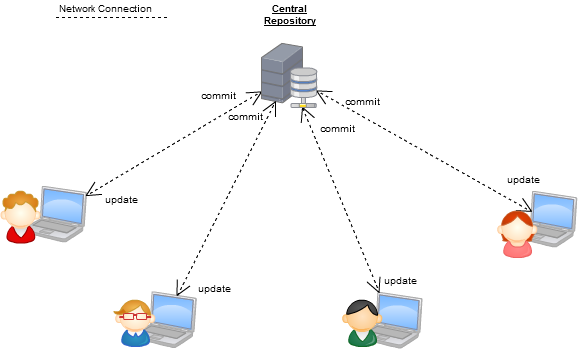
\includegraphics[width=\linewidth]{figs/centralized.png}
	\column{.50\linewidth}
	\centering Distributed (Git)\\\smallskip
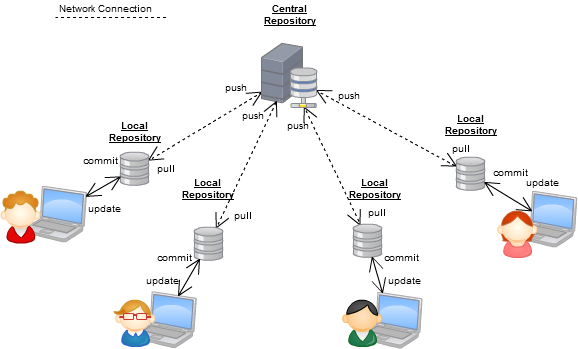
\includegraphics[width=\linewidth]{figs/distributed.png}
\end{columns}

\tiny \href{http://softwareengineering.stackexchange.com/questions/35074/im-a-subversion-geek-why-should-i-consider-or-not-consider-mercurial-or-git-or}{(Source)}
\end{center}
\end{frame}

%%%%%%%%%%%%%%%%%%%%%%%%%%%%%%%%%%%%%%%%%%%%%%%%%%%%%%%%%%%%%%%%%%%%%


\begin{frame}{Git}{Git vs. SVN (II)}
\begin{center}
\begin{columns}
	\column{.50\linewidth}
	\centering Fully distributed (Git)\\\smallskip
	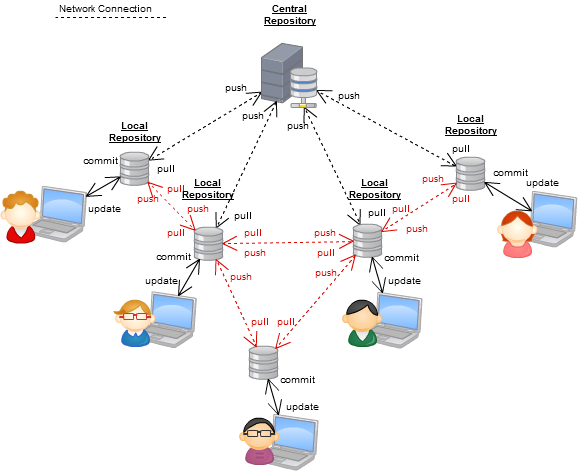
\includegraphics[width=\linewidth]{figs/fulldistributed.png}
	\tiny \href{http://softwareengineering.stackexchange.com/questions/35074/im-a-subversion-geek-why-should-i-consider-or-not-consider-mercurial-or-git-or}{(Source)}

	\column{.50\linewidth}
	\begin{block}{Git concepts to know}
	\begin{itemize}
	\item \texttt{commit}, \texttt{update}
	\item \texttt{push}, \texttt{pull}
	\item \texttt{origin}, \texttt{remote}
	\end{itemize}
	\end{block}
\end{columns}

\end{center}

\end{frame}


%%%%%%%%%%%%%%%%%%%%%%%%%%%%%%%%%%%%%%%%%%%%%%%%%%%%%%%%%%%%%%%%%%%%%%
\section{Using Git}

%%%%%%%%%%%%%%%%%%%%%%%%%%%%%%%%%%%%%%%%%%%%%%%%%%%%%%%%%%%%%%%%%%%%%%
\subsection{Repository initialization and clonning}

%%%%%%%%%%%%%%%%%%%%%%%%%%%%%%%%%%%%%%%%%%%%%%%%%%%%%%%%%%%%%%%%%%%%%%

\begin{frame}[fragile]{Using Git}{Basic commands: Repository initialization}

When using Git for the first time:

\begin{verbatim}
git config --global user.email user@uah.es
git config --global user.name  "Jane Doe"
\end{verbatim}

Initialization:

\begin{verbatim}
mkdir /path/to/your/project
cd /path/to/your/project
git init
git remote add origin https://<where>/<path>/<project.git>
git push -u origin --all # pushes up the repo and its refs for the first time
\end{verbatim}

\end{frame}

%%%%%%%%%%%%%%%%%%%%%%%%%%%%%%%%%%%%%%%%%%%%%%%%%%%%%%%%%%%%%%%%%%%%%%
\begin{frame}{Using Git}{Basic commands: Repository clonning}

To work with someone else’s repository, we first need to \emph{clone} it to get a
local copy.

\texttt{git clone <repo>}

E.g.:

\texttt{git clone https://github.com/danrodgar/gitSlides.git}

\begin{footnotesize}Note: once cloned, you can edit the repository as much as you want. No changes make their way back to the ‘central’ repository until you explicitly do so.
\end{footnotesize}
\end{frame}


%%%%%%%%%%%%%%%%%%%%%%%%%%%%%%%%%%%%%%%%%%%%%%%%%%%%%%%%%%%%%%%%%%%%%%
\subsection{Basic commands}


\begin{frame}[fragile]{Using Git}{Basic commands: tracking files}

Then, we can start tracking files. To do so, we need to \texttt{add}, \texttt{commit}, and \texttt{push} the file(s) that we want to track.


\begin{verbatim}
echo "A new file..." >> Readme.md
git add Readme.md
git commit -m 'Initial commit'
git push -u origin master
\end{verbatim}

\end{frame}


%%%%%%%%%%%%%%%%%%%%%%%%%%%%%%%%%%%%%%%%%%%%%%%%%%%%%%%%%%%%%%%%%%%%%%
\begin{frame}{Using Git}{Basic commands: Pulling}

% \begin{columns}
% 	\column{.50\linewidth}
% 	\centering Centralized (SVN)\\\smallskip
% 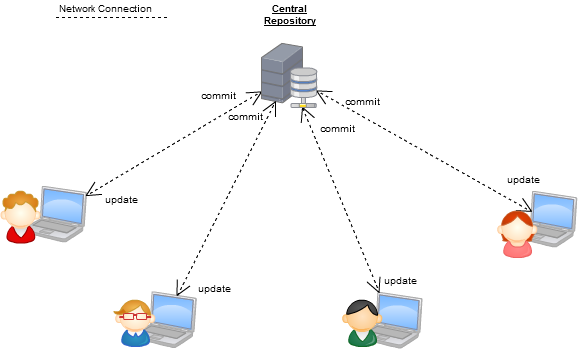
\includegraphics[width=\linewidth]{figs/centralized.png}
% 	\column{.50\linewidth}
% 	\centering Distributed (Git)\\\smallskip
% 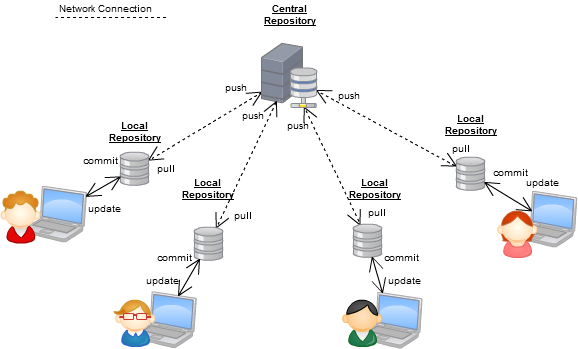
\includegraphics[width=\linewidth]{figs/distributed.png}
% \end{columns}
% To integrate all changes other people have made since you
% cloned/pulled: \texttt{git pull}

\begin{itemize}
 \item If you have made local changes you have to \\
 \texttt{git stash} \\
 before pulling, then \\
 \texttt{git stash pop} \\
 afterwards

 \item You can see which files you've modified with\\
  \texttt{git status}

 \item You can permanently remove your local changes by \\
 \texttt{git checkout <file>}
\end{itemize}

\end{frame}


%%%%%%%%%%%%%%%%%%%%%%%%%%%%%%%%%%%%%%%%%%%%%%%%%%%%%%%%%%%%%%%%%%%%%%
\begin{frame}{Using Git}{Basic commands: Pushing}

\texttt{git add <file>} makes git track the file <file>

Or to record all changes into a commit (notice the ‘.’):

\texttt{git commit .}

\texttt{git push origin master} This pushes all new commits to the repository.


\end{frame}


%%%%%%%%%%%%%%%%%%%%%%%%%%%%%%%%%%%%%%%%%%%%%%%%%%%%%%%%%%%%%%%%%%%%%%
\subsection{Merge and conflicts}
\begin{frame}{Using Git}{Merge and conflicts}

If two people both modify the same file, the first to push \emph{wins}.
The second person will have to pull and merge before pushing.

\begin{itemize}
 \item Changes in different parts of a file are automatically merged
 \item Changes in the same part of a file cause conflicts (between <<<
=== >>> ) and require the user to manually resolve them. Can
select either HEAD (your changes) or remote, or a mix of the two
\item Two merging cases: have / haven't committed
\end{itemize}

\end{frame}

%%%%%%%%%%%%%%%%%%%%%%%%%%%%%%%%%%%%%%%%%%%%%%%%%%%%%%%%%%%%%%%%%%%%%%
\begin{frame}{Using Git}{Merge and conflicts: \texttt{diff}}

\texttt{diff -u <old file> <new file>}

This command shows what changes you would need to apply to old file to change it into
new file.

Lines beginning with:
\begin{itemize}
 \item \texttt{- - -} or \texttt{+++} tell you the old / new filenames
 \item \texttt{@@} points to where within the file you are looking \\
       (i.e. a space) are lines that are unchanged
 \item \texttt{-} is a deleted line
 \item \texttt{+} is a newly added line
\end{itemize}

\end{frame}



%%%%%%%%%%%%%%%%%%%%%%%%%%%%%%%%%%%%%%%%%%%%%%%%%%%%%%%%%%%%%%%%%%%%%%
\begin{frame}[fragile]{Using Git}{Merge and conflicts: \texttt{diff} example}

\begin{scriptsize}
\begin{columns}
	\column{.50\linewidth}
	  \begin{verbatim}
	  #include <stdio.h>
	  int main() {
	    printf("Hello World\n");
	  }
	  \end{verbatim}
	\column{.50\linewidth}
	  \begin{verbatim}
	    #include <stdio.h>
	    int main(int argc, char *argv[]) {
	    printf("Hello World\n");
	    return 0;
	    }
	  \end{verbatim}
\end{columns}

Applying the \texttt{diff} command:
\begin{verbatim}
$ diff -u hello.c hello_new.c > hello.patch
\end{verbatim}

We get the following patch:
\begin{verbatim}
--- hello.c	2014-10-07 18:17:49.000000000 +0530
+++ hello_new.c	2014-10-07 18:17:54.000000000 +0530
@@ -1,5 +1,6 @@
 #include <stdio.h>
-int main() {
+int main(int argc, char *argv[]) {
 	printf("Hello World\n");
+	return 0;
 }
\end{verbatim}
\end{scriptsize}


\end{frame}

%%%%%%%%%%%%%%%%%%%%%%%%%%%%%%%%%%%%%%%%%%%%%%%%%%%%%%%%%%%%%%%%%%%%%%

\begin{frame}{Using Git}{Merge and conflicts: Applying \texttt{diff} changes (patch command)}

After the \texttt{patch.diff} is created as:

\texttt{diff -u <old file> <new file> > file.patch }

We can apply it with the \texttt{patch} command:

\texttt{patch < file.patch}

Note that the \texttt{file.patch} knows the name of the file to be patched.


\end{frame}

%%%%%%%%%%%%%%%%%%%%%%%%%%%%%%%%%%%%%%%%%%%%%%%%%%%%%%%%%%%%%%%%%%%%%%

\begin{frame}{Using Git}{Merge and conflicts: Original Patch!}

\centering
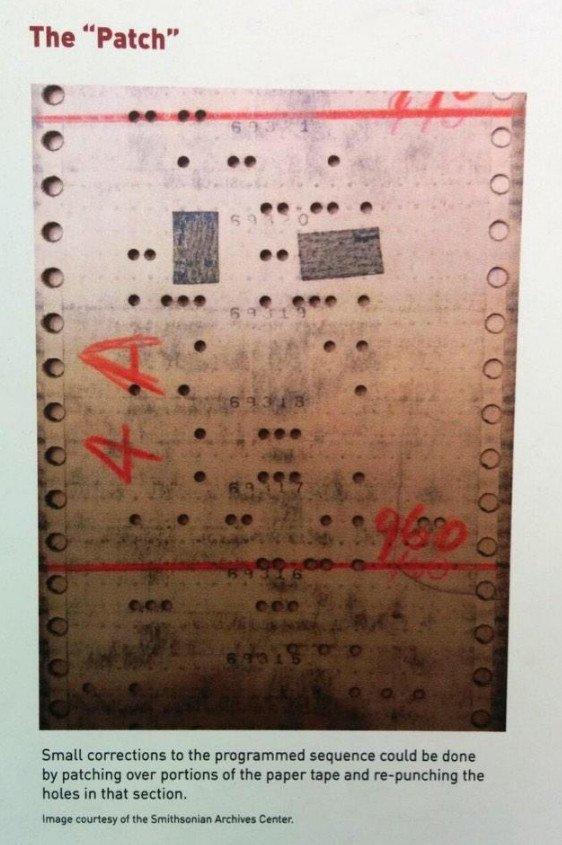
\includegraphics[width=.4\textwidth,height=\textheight,keepaspectratio]{figs/patch.png}

\end{frame}


%%%%%%%%%%%%%%%%%%%%%%%%%%%%%%%%%%%%%%%%%%%%%%%%%%%%%%%%%%%%%%%%%%%%%%
\begin{frame}{Using Git}{Commits}

\begin{itemize}
 \item Merge commits record where parallel development unified
 \item How does Git keep track of things when parallel development
happens?
\item Every commit has an ID (its hash), which is a 40 character SHA-1
hash based on the commit's content. Not guaranteed to be
unique; but it probably is
\end{itemize}

\end{frame}

%%%%%%%%%%%%%%%%%%%%%%%%%%%%%%%%%%%%%%%%%%%%%%%%%%%%%%%%%%%%%%%%%%%%%%
\subsection{Branches}
\begin{frame}{Using Git}{Branches}

Branches are used extensively (e.g. some like feature branches).

\begin{itemize}
 \item A repository (local and remote) can have explicit branches
 \item The default branch is called master
 \item \texttt{git branch <name>} creates branches
 \item \texttt{git checkout <branch name>} switch branches
 \item To merge branch X into Y, checkout Y and run git merge X
(i.e. you say “I want to merge another branch into me”)
\end{itemize}

\end{frame}

%%%%%%%%%%%%%%%%%%%%%%%%%%%%%%%%%%%%%%%%%%%%%%%%%%%%%%%%%%%%%%%%%%%%%%
% \subsection{Tags}
% \begin{frame}{Using Git}{Tags}
% 	TODO
% \end{frame}

%%%%%%%%%%%%%%%%%%%%%%%%%%%%%%%%%%%%%%%%%%%%%%%%%%%%%%%%%%%%%%%%%%%%%%
\subsection{Advanced Git}
\begin{frame}{Using Git}{Advanced Git: Getting an old commit}

Sometimes you need to get an old file or discard some changes. With

\begin{itemize}
 \item \texttt{git log}
 \item \texttt{git log -- oneline}
\end{itemize}

we can check previous commits and select one with \texttt{checkout}, e.g.:
\begin{itemize}
 \item \texttt{git checkout c71d008}
\end{itemize}

\end{frame}


%%%%%%%%%%%%%%%%%%%%%%%%%%%%%%%%%%%%%%%%%%%%%%%%%%%%%%%%%%%%%%%%%%%%%%
\begin{frame}{Using Git}{Advanced Git: Good practices}


Tipically changes are checked by someone other than their
author before being merged into master. This kind of \textbf{code review} is is naturally captured by pull requests in Git.

Learn on the job: the best way to learn it is by using it. However:
\begin{itemize}
  \item Best practice: regularly push and pull (at least daily, in general).
  \item Don't push half-baked changes or pull if you're in the middle of a task.
\end{itemize}

\end{frame}

%%%%%%%%%%%%%%%%%%%%%%%%%%%%%%%%%%%%%%%%%%%%%%%%%%%%%%%%%%%%%%%%%%%%%%

\section{GitHub}
\begin{frame}{GitHub}{GitHub}

\centering

\includegraphics[width=\textwidth,height=\textheight,keepaspectratio]{figs/github.png}


\end{frame}


% %%%%%%%%%%%%%%%%%%%%%%%%%%%%%%%%%%%%%%%%%%%%%%%%%%%%%%%%%%%%%%%%%%%%%%
% \begin{frame}{}
%
% \end{frame}
%


%%%%%%%%%%%%%%%%%%%%%%%%%%%%%%%%%%%%%%%%%%%%%%%%%%%%%%%%%%%%%%%%%%%%%%


\end{document}
